この場合はデータ自体に相関が存在すると、パラメタにも相関が存在し、パラメタを減らすことにより、パラメタ間の相関関係が解決し、最適解が収束する場合がある。
この時、このパラメタを減らすためにパラメタの絶対値の罰則項を付加することで、軸上に収束しやすくなり、パラメータを減らす収束値となる可能性がある正則化ができる。
この回帰をロッソ回帰といい、次の式で表される。
\begin{align*}
    {\rm min}\left\{ (D\mbox{\boldmath $w$}-\mbox{\boldmath $y$})^{T}(D\mbox{\boldmath $w$}-\mbox{\boldmath $w$})+\lambda \sum_{i=1}^{p} |w_{i}|\right\} \tag{2.3}
\end{align*}
また、これの場合は以下のようなデータがあり、以下のように通常なら、青色の線で識別するが、データ間に相関があるため、パラメタを一つ減らして、緑の線で識別できたり、赤色の線で識別できたりする。
\begin{center}
    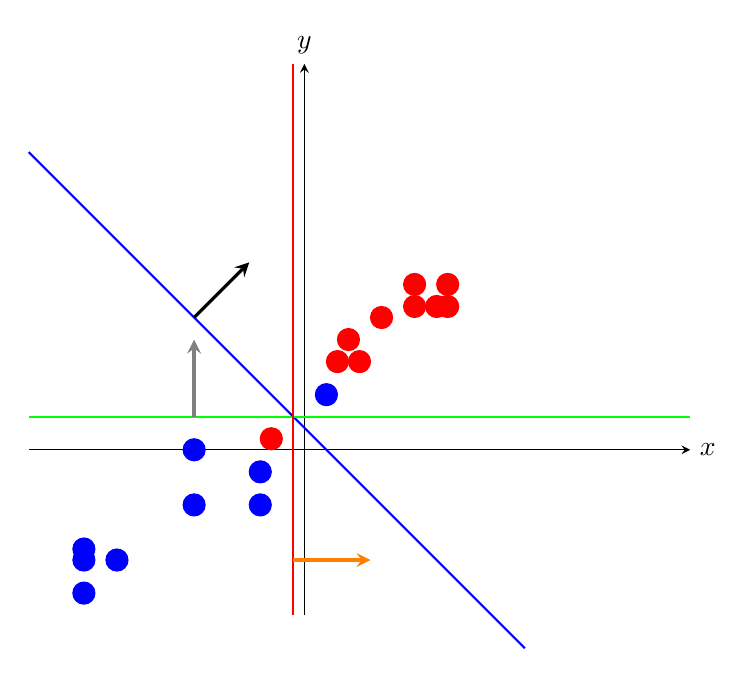
\begin{tikzpicture}[>=stealth,scale=1.4]
        \draw[->](-2.5,0)--(3.5,0) node[right] {$x$};
        \draw[->](0,-1.5)--(0,3.5) node[above] {$y$};
        \filldraw[fill=blue,draw=blue] (-1,0) circle[radius=0.1];
        \filldraw[fill=blue,draw=blue] (-1,-0.5) circle[radius=0.1];
        \filldraw[fill=blue,draw=blue] (-2,-1.3) circle[radius=0.1];
        \filldraw[fill=blue,draw=blue] (-1.7,-1) circle[radius=0.1];
        \filldraw[fill=blue,draw=blue] (-2,-0.9) circle[radius=0.1];
        \filldraw[fill=blue,draw=blue] (-2,-1) circle[radius=0.1];
        \filldraw[fill=blue,draw=blue] (-0.4,-0.2) circle[radius=0.1];
        \filldraw[fill=blue,draw=blue] (-0.4,-0.5) circle[radius=0.1];
        \filldraw[fill=red,draw=red] (-0.3,0.1) circle[radius=0.1];
        \filldraw[fill=red,draw=red] (0.4,1) circle[radius=0.1];
        \filldraw[fill=red,draw=red] (1.2,1.3) circle[radius=0.1];
        \filldraw[fill=red,draw=red] (1.3,1.5) circle[radius=0.1];
        \filldraw[fill=red,draw=red] (1.3,1.3) circle[radius=0.1];
        \filldraw[fill=red,draw=red] (1.0,1.5) circle[radius=0.1];
        \filldraw[fill=red,draw=red] (0.7,1.2) circle[radius=0.1];
        \filldraw[fill=red,draw=red] (0.5,0.8) circle[radius=0.1];
        \filldraw[fill=red,draw=red] (0.3,0.8) circle[radius=0.1];
        \filldraw[fill=blue,draw=blue] (0.2,0.5) circle[radius=0.1];
        \filldraw[fill=red,draw=red] (1,1.3) circle[radius=0.1];
        \draw[draw=blue,domain=-2.5:2.0,thick] plot(\x,{-1.0*\x+0.2});
        \draw[draw=black,->,very thick] (-1.0,1.2)--(-0.5,1.7);
        \draw[draw=green,thick] (-2.5,0.3)--(3.5,0.3);
        \draw[draw=gray,->,very thick] (-1.0,0.3)--(-1.0,1.0);
        \draw[draw=red,thick] (-0.1,-1.5)--(-0.1,3.5);
        \draw[draw=orange,->,very thick] (-0.1,-1.0)--(0.6,-1.0);
    \end{tikzpicture}
\end{center}
この場合はパラメタとして$\mbox{\boldmath $x$},\mbox{\boldmath $y$}$を使う必要はなく、$\mbox{\boldmath $x$}$だけでも識別可能な平面のパラメタとしては十分である場合がある。
そのため、このことを考慮に入れた最適化を行うために罰則項としてパラメタの絶対値を付加し、軸上に収束しやすくなる。